%Stil på uppsats
\documentclass[11pt]{article}
\usepackage[utf8]{inputenc}
\usepackage[swedish]{babel}
\usepackage{verbatim}
\renewcommand{\baselinestretch}{1.2}
\renewcommand{\arraystretch}{0.85}

\usepackage{makecell}
\setcellgapes{5pt}

\usepackage{tabularx}
\newcolumntype{Y}{>{\centering\arraybackslash}X}

%Skippa indrag av brödtext
\usepackage{parskip}

%Bilder sida vid sida
\usepackage{subfig}

% Formattera text
\usepackage[text={12cm,20cm}]{geometry}

\usepackage{booktabs}
\usepackage{floatrow}
\floatsetup[table]{capposition=top}
\usepackage{amsmath}
\usepackage{upgreek}
\usepackage{graphicx}
\graphicspath{{./images/}}
\usepackage{textgreek}
\usepackage{sectsty}

\numberwithin{equation}{section}
\numberwithin{table}{section}
\numberwithin{figure}{section}

\usepackage{titlesec}
\titleformat*{\section}{\Large\bfseries}
\titleformat*{\subsection}{\large\bfseries}
\titleformat*{\subsubsection}{\small\bfseries}



\usepackage[table,xcdraw]{xcolor}

\usepackage{afterpage}
\usepackage{sectsty}
\usepackage[labelfont=bf]{caption}
\usepackage{url}
\usepackage{hyperref}
\usepackage{array}
\usepackage{multirow}

% Bibliography
\usepackage[style=authoryear,sorting=nty]{biblatex} %Imports biblatex package
\addbibresource{references.bib} %Import the bibliography file

\usepackage[referable]{threeparttablex}
\usepackage{booktabs}
\usepackage{lipsum}

\usepackage[export]{adjustbox} %För titelsida


\begin{document}



\begin{titlepage}
\thispagestyle{empty}
	\begin{figure}[ht]
	   \minipage{0.7\textwidth}
			\includegraphics[width=4cm]{su2.jpeg}
			
	   \endminipage
	    \minipage{0.6\textwidth}
		 \Large Kandidatuppsats \par
		 \large Statisiska institutionen \par
		  \small Bachelor thesis, Department of   Statistics \par
		   \large Nr 2021:1 \par
			
\endminipage
\end{figure}
	
	
\centering
\vspace{5cm}

{\large\bfseries Tidsserieanalys av börsindex. En jämförelse mellan ARMA-GARCH och LSTM. eller nåt sånt....\par}
	\vspace{0.5cm}
	
{\large\itshape Time series analysis of stock index. A comparison between ARMA-GARCH and LSTM. \par}
	\vfill
	
	

{\Large Erik Billebjer Ulrikson och Erik Carle\par}
	\vspace{0.5cm}
	
\begin{flushleft}
Självständigt arbete 15 högskolepoäng inom Statistik III, VT2021 \\
Handledare: Ulf Högnäs\\

\end{flushleft}
\end{titlepage}


%%%%%%%%%%%% ABSTRACT %%%%%%%%%%%%%%%%%
\newpage
\thispagestyle{empty}
\section*{Sammanfattning}

I denna studie appliceras en LSTM (long short-term memory) på prisdata från OMX small-cap index som jämförs med den konventionella tidsseriemodellen ARIMA(1,1)-GARCH(1,1). Det visar sig att LSTM överträffar en ARMA(1,1) med GARCH(1,1) komponent på en periods sikt medan ARMA(1,1)-GARCH(1,1) ger mer exakta skattningar på 5, 21 och 63 dagars sikt. Vid simulerad handling över 1.000 perioder är ARMA(1,1)-GARCH(1,1) att föredra oavsett antal tidsperioder fram i tiden. Studien antyder att en ARMA(1,1)-GARCH(1,1) med fördel kan användas för att applicera en algoritmisk handelsstrategi som överpresterar index under den studerade perioden. 

\section*{Abstract}
In this study, an LSTM (long-term memory) is applied to price data from the OMX small-cap index as queries with the conventional time series model ARIMA (1,1)-GARCH (1,1). It turns out that LSTM outperforms an ARMA (1,1) with GARCH (1,1) component in one step ahead forecast while ARMA (1,1)-GARCH (1,1) gives more accurate estimates of 5, 21 and 63 days ahead. For simulated trading over 1.000 periods, ARMA (1,1)-GARCH (1,1) is preferred regardless of the number of time periods forecasted. The study suggests that an ARMA (1,1)-GARCH (1,1) can be used to apply an algorithmic trading strategy as it overperforms index during the period studied.


%%%%%%%%%%%% TABLE OF CONTENTS %%%%%%%%%%%%%%%%%
\newpage
\thispagestyle{empty}
{\fontsize{11pt}{11.5pt}\selectfont % making it fit in one page by adjusting baselineskip (the 2nd one)
    \tableofcontents
}
\thispagestyle{empty}
\newpage

%%%%%%%%%%%%%% Förkortningar %%%%%%%%%%%%%%%
\newpage 
\thispagestyle{empty}

\section*{Förkortningar}
\textbf{ADF-test} \dots Augmented Dickey-Fuller-test \par
\textbf{AIC} \dots Akaike Information Criterion \par
\textbf{ANN} \dots Artifical Neural Network \par
\textbf{ARCH} \dots Autoregressive Conditional Heteroskedasticity \par
\textbf{ARIMA} \dots Autoregressive Integrated Moving Average \par
\textbf{ARMA} \dots Autoregressive Moving Average \par 
\textbf{ARMA-GARCH} \dots Autoregressive Moving Average - Generalized Autoregressive Conditional Heteroskedasticity \par 
\textbf{BIC} \dots Schwarz Bayesian Information Criterion \par
\textbf{EMH} \dots Efficient Market Hypothesis \par
\textbf{GARCH} \dots Generalized Autoregressive Conditional Heteroskedasticity \par
\textbf{LM-test} \dots Lagrange Multiplier-test \par
\textbf{LSTM} \dots Long Short-Term Memory \par
\textbf{MAPE} \dots Mean Absolute Percentage Error \par
\textbf{OMXSSC} \dots OMX Stockholm Small Cap \par
\textbf{RMSE} \dots Root-Mean-Square Error \par
\textbf{RNN} \dots Recurrent Neural Network \par


\newpage
\thispagestyle{empty}

\begin{itemize}
    \item Abstract / Sammanfattning
    \item är det tydligt att t i tabellerna syftar till antal perioder framåt?
    \item vi ändrade ju kring precison, käsnlighet \& F-värde. var uppmärksam på om gamla resonemang mot förmodan ligger kvar
    \item tänk extra på att vi inte ska få det att låta som att vi testat LSTM mot ALLA ekonometriska modeller
    
    % Språkligt
    \item tempus (introduktion + teori = nutid, metod = nutid, resultat = nutid,  diskussion + slutsats = dåtid
    \item Bort: Man, vi, vår, prediktera, så, jag
    \item horungar
\end{itemize}

\newpage
%%%%%%%%%%%%%% INLEDNING %%%%%%%%%%%%%%%
\clearpage
\setcounter{page}{1}


\section{Inledning}
Efter att New York Stock Exchange började tillåta handel med hjälp av programvara på 1980-talet populariserades algoritmisk handel.  Idag sker en stor del av all handeln på finansmarknaden automatiskt med algoritmer, år 2012 utgjorde exempelvis algoritmisk handel 85 procent av marknadsvolymen på den amerikanska börsen \parencite[][,s.258]{glantz2013multi}. Denna utveckling har i stort sin grund i den breda utecklingen av avancerad programvara och ökade möjligheter att på ett enkelt sätt samla in och lagra stora mängder data. Detta är en uveckling som inte enbart småsparare dragit nytta av utan även de större aktörerna på marknaden som investmentbanker och hedgefonder \parencite{DE_Shaw}. Det har publicerats ett stort antal akademiska studier som visar på att algoritmer som använder artificiella neurala nätverk, så kallade djupinlärningsmodeller, istället för ekonometriska modeller (såsom ARIMA, GARCH mfl.) med fördel kan implementeras för att generera högre avkastning än index \parencite{paliwal2009neural}. En vanligt förekommande djupinlärningsmodell är LSTM (Long Short-Term Memory) som är en typ av neuralt nätverk med egenskapen att lära sig långsiktiga mönster i data, varför den ofta används just för tidsserieanalys inom kvantitativ finans.

Trots att det existerar ett brett segment av empirisk forskning på hur djupinlärningsmodeller med fördel kan användas finns det få studier som behandlar effekten av att implementera en sådan modell på ett svenskt index, vilket denna studie vill bidra med. Syftet med denna studie är således att undersöka om djupinlärningsalgoritmer med fördel kan användas istället för ekonometriska modeller på svenska börsindex. I denna studie besvaras följande frågor:

\begin{itemize}
    \item Kan en djupinlärningsmodell med fördel användas som substitut för en traditionell ekonometrisk modell på svenskt börsindex?
    \item Kan en algoritmisk handelsstrategi som ger högre avkastning utvecklingen hos ett svenskt småbolagsindex skapas?
\end{itemize}

Detta kommer utföras genom att jämföra LSTM med en ARIMA-modell med en GARCH-komponent, så kallad ARMA-GARCH. 

Denna studie är strukturerad på följande vis: I avsnitt 1.1 presenteras tidigare studier, i 1.2 avgränsningar, i avsnitt 2. presenteras finansiell teori, i avsnitt 3. presenteras teori kring de använda modellerna, i avsnitt 4. metoden och datamaterialet, avsnitt 5. presenterar resultatet, avsnitt 6. diskussionen och avsnitt 7. är slutsatsen. 

%%%%%%%%%%%%%% AVGRÄNSNINGAR %%%%%%%%%%%%%%%
\subsection{Avgränsningar}
Uppsatsen är begränsad till att enbart beröra småbolagsindex på Stockholmsbörsen och slutsatserna av analysen av vilken metod som är bäst går således inte nödvändigtvis att applicera på andra finansiella marknadsindex. Resultatet går inte heller nödvändigtvis att generalisera utanför de valda prediktionsperioderna.


%%%%%%%%%%%%%% TIDIGARE STUDIER %%%%%%%%%%%%%%%


\subsection{Relaterad forskning}

En av de mest omfattande studierna kring användandet av neurala nätverk i jämförelse med ekonometriska modeller genomfördes av Paliwal och Kumar \parencite*{paliwal2009neural}. I en metaanalys summerar de resultat från 96 studier inom olika områden och finner att neurala nätverk presterar lika bra och i många fall bättre än ekonometriska modeller. Det påpekas å andra sidan att en anledning till detta resultat kan bero på ouppfyllda antaganden kring de ekonometriska modellerna. 

I en annan studie som genomfördes av Namin \& Namin \parencite*{siaminamini2018forecasting} undersöker de hur väl LSTM och ARIMA predicerar ett flertal världsindex genom att jämföra spridningen av avvikelser i prediktionerna, och finner bevis för att LSTM överträffar ARIMA vad gäller förmågan att reducera prediktionsfel sett till storleken på RMSE. Qiu \& Song \parencite*{10.1371/journal.pone.0155133} finner likt Namin \& Namin \parencite*{siaminamini2018forecasting} att ett Artificellt Neuralt Nätverk (ANN) med fördel kan användas för att predicera framtida avkastning. Bollerslev (1986) presenterade GARCH som är en generaliserad variant av ARCH som presenterats bara några år innan av Engle (1982). Denna vidareutvecklade modell har visat sig 

%I en annan intressant studie som utfördes Jeong \& Lee \parencite*{jeong2019recurrent} applicerades en tangentfunkton i ARMA-komponenten och utifrån denna metod fann de bevis för att en modifierad icke-linjär ARMA-GARCH modell med liknande egenskaper som Recurrent Neural Network (RNN), predicerar framtida avkastning på S\&P500 mer precist än en ARMA-GARCH med linjära egenskaper. Detta är i linje med Long, Lu och Ciu \parencite*{long2019deep} och ges ytterliggare stöd av Sang \& Di Pierro \parencite*{sang2019improving} där de i en studie applicerar LSTM och visar på att utförandet av en trading-strategi baserat på ANN med fördel kan användas vid prediktion av finansiella tidsserier. 

Gemensamt för de flesta studier är att de jämför djupinlärningsmodeller med ARIMA, denna studie berör ARMA-GARCH på ett småbolagsindex med kortare prediktionsperioder och andra empiriska valideringsmetoder. Det finns ett flertal studier som berör storbolagsindex för ett enskilt land eller ett världsindex. Empiriska studier som jämför artificella nätverk gentemot en kombination av ARIMA och GARCH på svenska börsindex, synnerligen småbolagsindex, är mer sällsynt vilket denna studie vill bidra med. 

 

\newpage
%%%%%%%%%%%%%% FINANSIELL TEORI %%%%%%%%%%%%%%%
\section{Finansiell Teori}

\subsection{Hypotesen om effektiva marknader (EMH)}
Den effektiva marknadshypotesen, även känd som EMH, är en term som definerades första gången av Harry Roberts (1967) och utvecklades några år senare av Eugene Fama \parencite*{Fama1970} i artikeln \emph{"Efficient Capital Markets: A Review of Theory and Empirical Work"}. 

EMH är starkt förknippat med slumpvandring s.k. \emph{Random Walk}, som karakteriseras av en prisserie där alla efterföljande prisförändringar är slumpmässiga avvikelser från sin tidigare prisnivå. Om investerare har obehindrad tillgång till information och detta återspeglas direkt i prisnivån kommer morgondagens prisförändringar vara oberoende av dagens prisförändringar \parencite{EMH}. 

En marknad kan vara mer eller mindre effektiv baserat på tre former av marknadseffektivitet: \emph{Svag form}, \emph{halvsvag form} och \emph{stark form} \parencite{Fama1970}. \emph{Svag form} betyder att framtida priser omöjligt kan prediceras genom att analysera historisk data. \emph{Halvstark form} är en mer restriktiv variant som inkluderas av att all offentlig information redan reflekterats i priserna. I \emph{Stark form} inkluderas insiderinformation vilket gör den till den strängaste av de tre definitionerna med innebörden att dagens prisnivå återspeglar all information som finns tillgänglig.

På lång sikt menar förespråkare av EMH att majoriteten av investerare kommer misslyckas med att generera högre avkastning än marknaden eftersom det är hopplöst att finna en modell som är bättre än slumpvandring med drift. Således ges stöd för att en passiv strategi som utgår från att öppna en position och sedan behålla den är mest effektiv \parencite{EMHforecast}. EMH har dock kritiserats och delvis motbevisats \parencite{basu1977investment, ball1978anomalies}.

\subsection{Logaritmerad avkastning}

En avkastningserie besitter statistiska egenskaper som gör den mer lätthanterlig att arbeta med än en prisserie, varför denna typ av serie ofta används i finansiella studier. Låt $P_{t}$ vara priset på en tillgång vid tidpunkt $t$, bruttoavkastningen av en investering från tidpunkt $t$ till tidpunkt $t-1$ kan då defineras som

\begin{equation}
    1+R_{t} = \frac{P_{t}}{P_{t-1}}
\end{equation}


Kontinuerligt sammansatt avkastning, eller logaritmerad avkastning, har additiva egenskaper som innebär att avkastning kan adderas över tid.  Vid logaritmering reduceras även variationen och blir mer konstant över tid \parencite{tsay}. För att få fram den logaritmerade avkastningen logaritmeras  Avkastningen, låt $r_{t}$ definera den logaritmerade avkastningen vid tidpunkt $t$. Den logaritmerade avkastningen för period $t$ kan då formellt defineras som

\begin{equation}
    r_{t} = ln(1+R_{t}) = ln \Big( \frac{P_{t}}{P_{t-1}} \Big)
\end{equation}

Där $P_{t}$ är prisnivån vid tidpunkt $t$ och och $P_{t-1}$ är priset vid föregående period. 









\newpage
%%%%%%%%%%%%% METOD %%%%%%%%%%%%%%%%%%%%%%%%%%%
\section{Metod}
Nedan beskrivs metoden och datamaterialet. För att utföra statistiska test och skapa modeller har Python version 3.8 och R version 4.0 använts (se bilaga A). 

\subsection{Stationäritet}
Stationäritet är centralt vid analys av tidsserier. En väsentlig egenskap hos stationära tidsserier är att de inte påverkas av stora temporära förändringar (s.k. chocker) över tid, utan dessa effekter försvinner relativt snabbt. I en icke-stationär tidsserie förblir chocker och påverkar framtida värden på tidsserien. Detta i sin tur gör att många statistiska test inte längre är giltiga, bl.a. t-test. \parencite[][,s.329 f.]{montgomery2015forecasting}. \par

I strikt mening innebär stationäritet att tidsserien uppvisar liknande 'statistikt beteende' över tid. Vanligtvis används dock svag stationäritet, vilket definieras som 1) tidsseriens förväntade värde beror inte på tid, \(E(y_t)=\mu_y\) och 2) autokovariansfunktionen är enbart en funktion av k och inte tid, \(\gamma_y(k) = Cov(y_t, y_{t+k})\) (ibid). För att illustrera stationäritet visar Figur 3.1 en typiskt stationär och en typiskt icke-stationär tidsserie.

\begin{figure}[H]
\caption{Illustration av stationäritet med simulerad data}
\includegraphics[width=0.9\linewidth]{stationarity.png}
\centering
\end{figure}

För att testa stationäritet används augmented Dickey-Fuller-test (ADF-test). Nollhypotesen är att en enhetsrot finns, \(\phi=1\) och alltså ingen stationäritet. Alternativhypotsen är att \(\phi<1\). Definiera \(\theta = \phi -1 \) för att kunna testa \(H_0:\theta=0\) i en regression. Låt \(y_t\) vara beroende variabeln, \( \alpha \) en konstant, \( \gamma \) en koefficient, \(e\) är felterm och p antal laggar \parencite[][,s.610 ff.]{wooldridge2018introductory}. Formeln är som följer:

\begin{equation}
    \Delta y_t = \alpha + \theta y_{t-1} + \gamma_1\Delta y_{t-1} + ... + \gamma_p\Delta y_{t-p} + e_t
\end{equation}
\begin{equation}
        = \alpha + \theta y_{t-1} + \sum_{t=1}^{p}\gamma_p \Delta y_{t-p} + e_t
\end{equation}

Om \(\theta\) är skild från noll förkastas alltså nollhypotesen att ingen stationäritet finns.

\subsection{Heteroskedasticitet}

Eftersom denna uppsats applicerar ARIMA med en GARCH-komponent behöver det testas att en ARIMA-modell ger heteroskedastiska residualer, annars finns ingen anledning att inkludera GARCH-komponenten. För att testa detta används Lagrange Multiplier-test (LM-test) som utgår från att modellera bästa möjliga AR-modell för att sedan modellera en regression på de kvadrerade feltermerna \(e_t^2\). Regressionen består av en konstant \(\alpha_0\) och laggade feltermer \(e_{t-i}\) enligt

\begin{equation}
    e_t^2=\alpha_0+\sum_{i=1}^{p}\alpha_ie_{t-i}^2
\end{equation}

Nollhypotesen är att alla \(\alpha_i\) = 0, vilket tyder på avsaknad av GARCH-komponenter i feltermen och att homoskedasticitet föreligger. Alternativhypotesen är att heteroskedasticitet föreligger och därför att det finns belägg för att använda en GARCH-komponent \parencite{engle1982autoregressive}. 

\subsection{Val av optimal modell}
En statistika behövs för att avgöra vilka parametervärden som är optimala. Två vanligt förekommande sådana mått är Akaike Information Criterion (AIC) samt Schwarz Bayesian Information Criterion (BIC). Modellen i fråga bestraffas för att inkludera ytterligare parametrar, vilket alltså gör AIC och BIC perfekt för att exempelvis hitta optimalt antal laggar. Låt $T$ vara antal observationer, $e$ felterm och $p$ antal parametrar \parencite[][s.76 f.]{montgomery2015forecasting}:
\begin{equation}
    AIC = ln\left( \frac{\sum_{t=1}^{T}e^2_t}{T} \right)+\frac{2p}{T}
\end{equation}
\begin{equation}
    BIC = ln\left( \frac{\sum_{t=1}^{T}e^2_t}{T} \right)+\frac{ln(T)p}{T}
\end{equation}

I både AIC och BIC indikerar lägre värden mer optimal modell. 

\subsection{ARMA-GARCH}
För att hantera heteroskedasticitet i tidsserier utvecklades ARCH och GARCH av Engle \parencite*{engle1982autoregressive} respektive Bollerslev \parencite*{bollerslev1986generalized}. Genom att kombinera ARMA och GARCH till en hybridmodel, ARMA-GARCH, går det att fånga systematiska skillnader i medelvärdet av tidsserien över tid med ARMA-komponenten såväl som systematiska skillnader i varians med GARCH-komponenten. Modellen är relativt ny inom men har blivit populär inom flera olika områden \parencite{chen2011short}. 

Nedan följer formeln för modellen. \(e_t\) är felterm, \(\delta\) en konstant, \(\phi_i\) vikter för laggade beroende variabel i AR(p), \(\theta_i\) vikter för laggade feltermen i MA(q), \(z_t\) är oberoende och identiskt fördelad med väntevärde 0 och varians 1, w en konstant, \(\alpha_i\) vikt för ARCH-termen och \(\beta_i\) vikt för GARCH-termen \parencite[][,s.507 ff.]{bollerslev1986generalized, montgomery2015forecasting}.

\begin{equation}
    y_t = \delta + \sum_{i=1}^{p}\phi_iy_{t-i}  +e_t - \sum_{i=1}^{q}\theta_i e_{t-i} 
\end{equation}
\begin{equation}
    e_t=\sqrt{\sigma_t^2}*z_t,\quad \sigma^2_t=w + \sum_{i=1}^{q}\alpha_i e^2_{t-i} + \sum_{i=1}^{p}\beta_i \sigma^2_{t-i}
\end{equation}

Förenklat uttryckt modellerar alltså ARMA den beroende variabeln i ekvation 3.6 och GARCH feltermern i ekvation 3.7. 

Vid specificeringen av ARMA-GARCH modellen testas först att modellens antagnaden är uppfyllda. Med Augmented Dickey-Fuller-test avgörs om tidsserien är stationär. Här används en funktion  i R (\textit{ur.df}) som optimalt väljer antal tidslaggar baserat på AIC innan testet utförs.  För att bekräfta att det specifierade antalet laggar genererar en modell med oberoende residualer görs därefter ett Ljung-Box-test med nollhypotesen att residualerna är oberoende och alternativhypotesen att de inte är oberoende \parencite{box1970distribution}. En annan förutsättning är att feltermerna av en ARIMA är heteroskedastiska, därför görs det tidigare nämnda Lagrange Multiplier-testet på bästa möjliga ARIMA-modell. Givet att det inte finns belägg för homoskedasticitet väljs sedan bästa möjliga ARMA-GARCH-modell utifrån AIC och BIC. 


\subsection{Long Short-Term Memory (LSTM)}
LSTM är en typ av upprepat neuralt nätverk (RNN: Recurrent Neural Network), vilket i sin tur är en sorts artificiellt neuralt nätverk (ANN). En väsentlig fördel med att använda artificiella neurala nätverk framför mer traditionella statistiska metoder är att de automatiskt kan approximera icke-linjära matematiska funktioner som är komplexa att hantera statistiskt \parencite{paliwal2009neural}. Således kan LSTM tänkas identifiera mönster som ARMA-GARCH inte har förmågan att identifiera.  För att förstå LSTM behövs en grundläggande förståelse för artificiella neurala nätverk. 

Ett artificiellt neuralt nätverk är en struktur av sammankopplade neuroner inspirerad av biologiska neurala nätverk. Nätverket består av flertalet olika algoritmer som tillsammans utför beräkningar. RNN är artificiella neurala nätverk som är särskilt bra på att hantera temporär data. Till skillnad från vanliga artificiella nätverk har varje neurons celler ett 'minne', där all indata behandlas i loopar. På detta sätt kan de 'komma ihåg' tidigare data. Dock inte särskilt länge, vilket är varför LSTM behövs \parencite[][,s.478-559]{purkait2019hands}. 

LSTM-nätverk kan behålla information i ett långsiktigt minne (en: \textit{state}), som förs över mellan tidsperioder. En LSTM-cell ser ut som följer i Figur 3.2:
\begin{figure}[H]
\caption{LSTM-cellens struktur \parencite[lånad från][]{yuan2019nonlinear}}
\includegraphics[width=10cm]{lstm.png}
\centering
\end{figure}

Varje LSTM-cell har tre indata; det långsiktiga minnet från tidigare steg \(c_{t-1}\), indatan från tidigare steg \(h_{t-1}\) och den nya indatan \(x_{t}\).

Först kommer \textit{forget gate}, det är den som gör att LSTM skiljer sig från RNN. Detta eftersom forget gate bestämmer huruvida indatan från tidigare steg (\(h_{t-1}\)) ska behållas eller förkastas från det långsiktiga minnet. Beslutet görs baserat på värdet i förra tidsperioden och den nya indatan, genom att ge olika vikter mellan 0 och 1 (där 1 är högst vikt). \textit{Input gate} kontrollerar flödet av information i det befintliga cellminnet. Denna grind bestämmer vilken ny information som ska läggas till i det långsiktiga minnet. I den sista grinden, \textit{output gate}, avgörs vad som ska läggas till i det 'dolda' långsiktiga minnet (en: hidden state) (\(h_{t}\)) inför nästa tidsperiod.

Varje neurons cell tar alltså emot tre indata och skickar vidare två utdata till nästa cell. Detta itereras sedan över alla datapunkter och efter den sista iterationen omvandlas det dolda långsiktiga minnet till utdata i önskat format \parencite[][,s.478-559]{purkait2019hands}.

Väldigt förenklat kan det alltså förklaras som  att för varje tidpunkt i datan skickas datan in i LSTM-cellerna, itereras i dessa där det avgörs vad som ska tas med i beräkningarna av nästa datapunkt $(t+1)$, itereras sedan över alla datapunkter och till slut görs prediktioner baserat på modellen. 

Definiera \(x_t\) som indatavektorn, \(f_t\) som forget gates aktiveringsvektor, \(i_t\) input gates aktiveringsvektor, \(O_t\) output gates aktiveringsvektor, \(h_t\) det dolda långsiktiga minnets vektor (även kallad utdatavektorn), \(\tilde{c_t}\) cellens indataaktiveringsvektor, \(c_t\) cellens långsiktiga minnes-vektor, \(W, U, b\) vikt- och biasmatriser som modellen lär sig under träning. \(\sigma\) är sigmoidfunktion och tanh hyperbolisk tangentfunktion. Cirklarna representerar elementvis produkt. Nedsänkt i hänvisar till input gate, nedsänkt o till output gate, nedsänkt f till forget gate, c till minnescellen och t till tidpunkt \parencite[][,s.478-559]{purkait2019hands}. Nedan styr ekvation 3.8 vad som händer i forget gate, 3.9 input gate och 3.10 output gate. I 3.11 kombineras dessa tre ekvationer, i 3.12 skapas utdatan och den multipliceras sedan med det befintliga dolda långsiktiga minnet i 3.13.

\begin{equation}f_t = \sigma(W_f x_t + U_f h_{t-1} + b_f)\end{equation}
\begin{equation}i_t = \sigma(W_i x_t + U_i h_{t-1} + b_i)\end{equation}
\begin{equation}o_t = \sigma(W_o x_t + U_o h_{t-1} + b_o)\end{equation}
\begin{equation}\tilde{c}_t = tanh(W_c x_t + U_c h_{t-1} + b_c)\end{equation}
\begin{equation}c_t= f_t \circ c_{t-1} + i_t \circ \tilde{c}_t\end{equation}
\begin{equation}h_t= o_t \circ tanh(c_t)\end{equation}

LSTM har inga formella antaganden och därav finns inga formella test att tillgå. Modellen utformas efter ett implicit antagande att det långsiktiga minnet från en period beror på det långsiktigta minnet från perioden innan. Det vill säga att det långsiktiga minnet kan överföras mellan tidsperioderna. Det behövs inte heller någon särskild distribution eftersom det neurala nätverket lär sig träningsdatans empiriska distribution \parencite[][,s.478-559]{purkait2019hands}.

För att skatta en LSTM behöver modellen så kallade hyperparametrar. Dessa hyperparametrar är olika för olika modeller och alla behöver inte specifieras. Ämnet är relativt outforskat, nedan följer de parametrar där det finns studier på hur de bör specifieras. Övriga parametrar väljs utifrån vad som är vanligt förekommande. Antal laggar väljs till lika många som i ARMA-GARCH för jämförbarhetens skull.

Hyperparametrarna med gedigen forskning bakom sig är \textit{förlustfunktion, optimeringsalgoritm} och antal \textit{epoker}.

Förlustfunktionen ger ett mått på hur väl modellen presterar på träningsdatan. Den används som ett mått på modellens fel och detta ska minimeras. MSE (Mean Square Error) rekommenderas för de flesta 'regressionsliknande' modeller, och därför även i detta fall \parencite[][,s.178 ff.]{purkait2019hands}. \par
Optimeringsalgoritm är den typ av algoritm som används för att minimera det ovan beskrivna felet. 'Adam' är en optimeringsalgoritm som visat sig fungera bra för stora dataset och rekommenderas av Purkait \parencite*[][,s.178 ff.]{purkait2019hands}. \par
Epoker indikerar antal gånger modellen kommer att itererar genom hela datasetet. Tidigare studier har kommit fram till att valet inte har någon relevant betydelse för hur väl modellen presterar \parencite{siaminamini2018forecasting}. Då Purkait använder fem epoker för LSTM, använder även denna uppsats fem \parencite[][,s.178 ff.]{purkait2019hands}. \par


\subsection{Validering}
\subsubsection{RMSE och MAPE}
För att mäta hur mycket de skattade stängningspriserna avviker från de verkliga stäningspriserna används RMSE (Root Mean Square Error), som ett mått på medelvärdet av standardfelen. Den bärande egenskapen hos RMSE är att större prediktionsfel får relativt större vikt då måttet baseras på ett viktat medelvärde enligt

\begin{equation}
RMSE = \sqrt{\frac{1}{n}\sum_{i=1}^{n}   (\hat{\theta_{t}} - \theta_{t})^2}
\end{equation}

där \emph{n} är det totala antalet observationer, $\theta_{t}$ är den faktiska prisnivån och $\hat{\theta_{t}}$ är den skattade prisnivån under handelsdag \emph{t}. 

Utöver RMSE används även MAPE (Mean Absolute Percentage Error) som har liknande egenskaper som RMSE men mäter de absoluta avvikelserna relativt nivån hos $\theta$, vilket ger de relativa avvikelserna i procent enligt

\begin{equation}
    \textit{MAPE}=\frac{1}{n} 
    \sum_{t=1}^{n} \left| \frac{\theta_{t}-\hat{\theta}_{t}}{\theta_{t}} \right| * 100
\end{equation}

Den främsta fördelen med MAPE jämfört med RMSE är att den är enklare att tolka tack vare att den är relativ. 




\subsubsection{Precision, känslighet och F-värde}
För att mäta hur väl modellerna predicerar en stigande respektive fallande prisnivå används en sammanblandningsmatris (en. \textit{confusion matrix}) som registrerar antalet korrekta och inkorrekta klassifikationer \parencite{ModelValidation}. I Tabell 3.1 syns en sammanblandningsmatris för den binära klassifikationen.

{    % for making group where "\makegapedcells" is valid
\makegapedcells
\begin{table}[H]
\caption{Sammanblandningmatris}
\begin{tabular}{cc|cc}
\multicolumn{2}{c}{}
            &   \multicolumn{2}{c}{Prediktion}                      \\
    &       &   \emph{Stigande} &  \emph{Fallande}              \\ 
    \cline{2-4}
\multirow{2}{*}{\rotatebox[origin=c]{90}{Faktisk}}
    & \emph{Stigande}   & Sann stigande (SS)   & Falskt fallande (FF)                 \\
    & \emph{Fallande}    & Falskt fallande (FS)    & Sann fallande (SF)                \\ 
    \cline{2-4}
    \end{tabular}
    \end{table}
 }

Tre mått relaterade till sammanblandningsmatrisen är precision, känslighet och F-värde. Måtten ger tillsammans en insikt över hur exakt modellen är. Precision ger svar på frågan 'Hur stor andel av predicerade positiva stiganden är korrekta?' och mäts enligt
\begin{equation}
    \textit{Precision} = \frac{\sum(SS)}{\sum(SS)+\sum(FS)} 
\end{equation}

Känslighet ger svar på frågan 'Hur stor andel av de predicerade uppgångarna var korrekt identifierade?'. Notera att skillnaden mot precision är att precision mäter 'givet att prediktionen var ökat värdet, gick värdet upp?' medan känslighet mäter 'givet att värdet har ökat, var prediktionen korrekt?'. Känslighet mäts genom att dividera antalet korrekt skattade stigande prediktioner med det totala antalet stigande prisnivåer enligt

\begin{equation}
    \textit{Känslighet} = \frac{\sum(SS)}{\sum(SS)+\sum(FF)}
\end{equation}

$F_{\beta}$-värdet är ett mått på exakthet där ett positivt värde ges till faktorn $\beta$ för att värdera antingen precision eller känslighet högst, detta värde defineras som

\begin{equation}
    F_{\beta} = \frac{(\beta^2+1) \textit{Precision} * 
    \textit{Känslighet}}{\beta^2  \textit{Precision} + \textit{Känslighet}}
\end{equation}

För att ge ett balanserat mått viktas precision och känslighet lika med $\beta=1$ \parencite{ModelValidation}. Ett harmoniskt medelvärde mellan de två måttes fås då enligt

\begin{equation}
    \textit{F1} = 2 \Big( \frac{\textit{Precision} * \textit{Känslighet}}{\textit{Precision} + \textit{Känslighet}} \Big)
\end{equation}

Där $F1=1$ är det högsta värdet som indikerar optimal precision och känslighet, medan $F1=0$ är det lägsta värdet och indikerar att precision eller känslighet är noll.


\subsubsection{Korsvalidering}
Tidsserien korsvalideras med en k-delad korsvalidering som innebär att träning- och testdata flyttas en period framåt från dess ursprungliga startpunkt i $n$ perioder, en procedur som visualiseras nedan i Figur 3.3. Vid nästa period inkluderas alltså det första värdet som predicerades mot i nya träningsdatan \parencite{bergmeir2018note}. I denna studie utförs korsvalideringen över 1.000 perioder. 

\begin{figure}[H]
\caption{Illustration av k-delad korsvalidering med fyra perioder.}
\includegraphics[width=0.9\linewidth]{cross_validation.png}
\centering
\end{figure}


Fördelen med denna typ av korsvalidering är att prediktioner görs vid 1.000 olika punkter istället för att utgå från en enstaka punkt. Att 1.000 perioder görs möjliggör även medelvärdesanalys av valideringsmåtten och en statistisk jämförelse mellan dem. För att jämföra måttens medelvärden används z-test då antalet observationer, $n=1.000$, ses som tillräckligt.

Låt $a$ motsvara ARMA-GARCH och $b$ LSTM, $i$ vara det valideringsmått som testas och $t$ antal perioder som prediceras framåt i tiden. Då är $\Bar{a}_{i,t}$ ARMA-GARCHs medelvärde för valideringsmått $i$ vid $t$ perioders prediktion, $s_{a,i,t}^2$ variansen och $n_a$ antal observationer. På samma sätt är  $\Bar{b}_{i,t}$ LSTMs medelvärde för valideringsmått $i$ vid $t$ perioders prediktion, $s_{b,i,t}^2$ variansen och $n_b$ antal observationer. Notera dock att $n_a = n_b$. Hypoteserna är som följer. Valet av alternativhypotes beror på om det testas om ARMA-GARCH är högre än LSTM (ekvation 3.21) eller tvärtom (ekvation 3.22) för ett givet valideringsmått vid en given prediktionsperiod. 

\begin{equation}
    H_0: \Bar{a}_{i,t} - \Bar{b}_{i,t} = 0 \Leftrightarrow \Bar{a}_{i,t} = \Bar{b}_{i,t}
\end{equation}
\begin{equation}
    H_1: \Bar{a}_{i,t} - \Bar{b}_{i,t} > 0
\end{equation}
\begin{equation}
    H_1: \Bar{a}_{i,t} - \Bar{b}_{i,t} < 0
\end{equation}

Teststatistikan är: 

\begin{equation}
    z = \frac{\Bar{a}_{i,t} - \Bar{b}_{i,t} - 0}{\sqrt{\frac{s_{a,i,t}^2}{n_a}+\frac{s_{b,i,t}^2}{n_b}}} \sim N(0,1)
\end{equation}
Som sedan jämförs med det kritiska värdet 1,64 för ett ensidigt test på 5\% signifikansnivå.


\subsubsection{Handelsstrategi}
För att undersöka hur väl modellerna presterar när de appliceras för att handla med simuleras en handelsstrategi över samma 1.000 perioder som i korsvalideringen. I simuleringen är en enhet av index utdistribuerat att handla med. Handeln utförs baserat på prediktioner på 1, 3, 5, 21 och 63 dagars sikt. Vid varje dag under de 1000 dagarna görs alltså prediktioner 1, 3, 5, 21 och 63 dagar fram i tiden och baserat på vad prediktionen är tas ett beslut. Följande strategier används:

\begin{itemize}
    \item Lång strategi: Strategin baseras på att automatiskt öppna en lång position (lägga en köporder) när modellen predicerar att prisnivån $t$ dagar fram kommer att vara högre än vid tidpunkten då prediktionen görs ($t=0$). Med andra ord görs ett köp om $P_t > P_0$.
    \item Kort strategi: Gå kort (lägga en säljorder) när modellen predicerar att prisnivån $t$ dagar fram kommer att vara lägre än tidpunkten då prediktionen görs ($t=0$). Med andra ord görs ett sälj om $P_t < P_0$.
    \item Behållstrategi: Behålla (varken köpa eller sälja) om det predicerade priset är identiskt med priset då prediktionen görs, dvs. $P_t = P_0$, eller om den föreslagna ordern är identisk med ordern innan. Det senare eftersom det bara går att äga en enhet av indexet åt gången. Exempelvis blir två köpindikationer på rad således ett köp och ett håll.
\end{itemize}

Modellerna jämförs i sin tur med en passiv strategi - att öppna en lång position i index och behålla den utan ytterliggare handlingar. Om LSTM och ARMA-GARCH lyckas spekulera rätt kring uppgångar och nedgångar om den framtida prisnivån kommer de i snitt generera högre avkastning än den passiva strategin. 

\newpage
\section{Datamaterial}

Data på dagliga stängningspriser för småbolagsindexet OMX Stockholm Small Cap (OMXSSC) hämtas från Refinitiv Eikon som är ett finansiellt system och används av över 40 000 institutioner världen över \parencite{Eikon}. Datan omfattar perioden 1 januari 2003 (när indexet skapades) till 12 februari 2021. I OMXSSC inkluderas data från totalt 93 svenska småbolag, vilka defineras som bolag med ett börsvärde som understiger 150 miljoner euro \parencite{smabalagsdefinition}. Bilaga B specificerar alla bolag som ingår OMXSSC. I \emph{Figur 4.1} samt \textit{Tabell 4.1} ges en överblick av stängningspriserna under perioden. 

\begin{figure}[H]
\caption{Prisserie över OMXSSC}
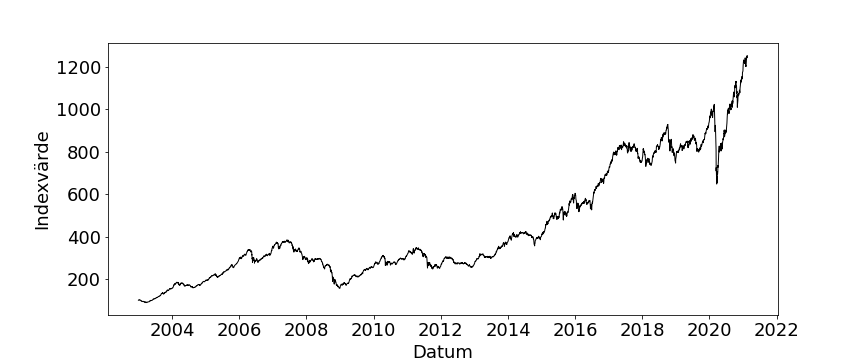
\includegraphics[width=\linewidth]{index.png}
\centering
\end{figure}


\begin{table}[H]
\caption{Deskprivtiv statistik över priser i OMXSSC}
\resizebox{\columnwidth}{!}{
\begin{tabular}{@{}llllllllll@{}}
\cmidrule(r){1-8}
%
Index  & Start      & Slut       & N    & Min.    & Medelvärde & Max.     & SD  \\ \cmidrule(r){1-8}
OMXSSC & 2003-01-01 & 2021-02-14 & 4564 & 88,54 & 436,45   & 1254,09 & 264,05  \\ \cmidrule(r){1-8}
\end{tabular}}
\end{table}

I Figur 4.2 syns den logaritmerade avkastningsserien där perioder med hög volatilitet kännetecknas av aggressiva prisförändringar. I Tabell 4.2 visas sedan deskriptiv statistik. 

\begin{figure}[H]
\caption{Logaritmerad avkastningsserie över OMXSSC}
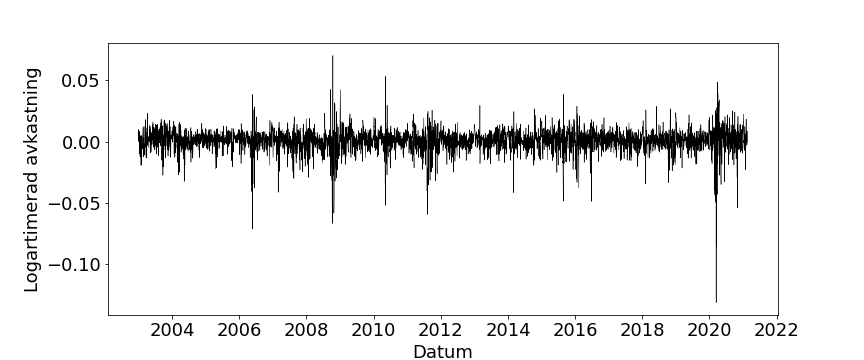
\includegraphics[width=\linewidth]{logreturns.png}
\centering
\end{figure}



\begin{table}[H]
\caption{Deskriptiv statistik över logaritmerad avkastning i OMXSSC}
\begin{tabular}{@{}llllllllll@{}}
\cmidrule(r){1-7}
%
Index  & Min.    & Medelvärde & Max    & SD     & Skrevhet & Kurtosis \\ \cmidrule(r){1-7}
OMXSSC & -0,0875 & 0,0056     & 0,0701 & 0,0006 & -1,4438  & 12,9149  \\ \cmidrule(r){1-7}
\end{tabular}
\end{table}






Eftersom logaritmerade priser kan ses som svårtolkade transformeras dessa om till prisnivå efter att modellen gjort sina skattningar. Den kumulativa summan av den logaritmerade avkastningen under period $t$ exponentieras enligt

\begin{equation}
    \text{Prisnivå} =  exp\Big({\sum\limits_{t=1}^n \hat{\theta_{t}}} + ln(\phi)\Big)
\end{equation}

Där  $\hat{\theta_t}$ är predicerad logaritmerad avkastning för tidpunkt $t$ och $\phi$ är träningsperiodens sista datapunkt. 


%forecasted_price = exp(cumsum(forecast) + log(last_train))

% Denna känns lite mis placé 
%Skevhetskoefficienten för avkastningsserien är negativ - fördelningen har en lång negativ svans med större frekvens av negativa avkastningar jämfört med positiva avkastningar. Kurtosiskoefficienten är större än tre och kännetecknas av en tjock svans (En: "\emph{fat tail}") där dagar med onormalt hög avkastning förekommer mer frekvent än hos en normalfördelning.

Prediktioner görs $(t=1, 3, 5, 21, 63)$ dagar fram i tiden, där $t=1$ är en börsdag,  $t=3$ motsvarar en halv börsvecka, $t=5$ en hel börsvecka, $t=21$ en börsmånad och $t=63$ ett börskvartal. Vidare delas 75 procent av datamaterialet in i träningsdata som sträcker sig från 1 januari 2003 till 31 juli 2016. Resterande del av datamaterialet utgörs av testdata som sträcker sig mellan den 3 augusti 2016 till den 14 febuari 2021. 

\newpage
%%%%%%%%%%%%%% RESULTAT %%%%%%%%%%%%%%%
\section{Resultat}
\subsection{ARMA-GARCH modellvalidering}
Först och främst testas om tiddserien är stationär med hjälp av Augmented Dickey-Fuller-test (ADF-test). Det är signifikant med $p<0,01$, optimalt antal laggar var 1 (se bilaga C). Nollhypotesen att tidsserien inte är stationär förkastas alltså. Således behövs ingen differentiering i ARIMA, dvs. en ARIMA(p,0,q)=ARMA(p,q) är tillräcklig. För att validera om feltermen behöver modelleras med GARCH eller om det räcker med en ARIMA-modell väljs först den optimala ARIMA-modellen (sett till datasetet) utifrån AIC med hjälp av funktionen \textit{auto.arima} i R. Detta ger en ARIMA(1,0,1), i tabell 5.1 följer en sammanställning över denna. För att säkerställa oberoende i feltermerna för modellen gjordes ett Ljung-Box-test. Detta visar att residualerna i ARIMA-modellen inte är beroende (se bilaga D). Slutligen testas efter heteroskedasticitet i ARIMA-modellen med LM-test. Nollhypotesen förkastas, $p=0.00$, och alltså visas tydliga tecken på heteroskedasticitet (se bilaga E). Detta indikerar att feltermen egentligen bör modelleras med GARCH. 

\begin{table}[H]
\caption{Sammanfattning av ARIMA(1,0,1)}
\begin{tabularx}{\textwidth}{c *{6}{Y}}
\toprule

Parameter  & Skattning & Standardfel & p-värde \\
\hline

$\delta$        & 0,0005  & 0,0002  & $0,0087$   \\
$\phi_1$        & 0,6737  & 0,0670  & $<2,2*10^{-16}$   \\

$\theta_1$      & -0,5574 & 0,0754  &  $1,42*10^{-13}$   \\
\midrule

Informationskriterier  & &  &  \\
\hline

Log likelihood        & 11.358,46 \\
AIC                   & -22.708,91 \\

BIC                   & -22.683,36 \\
\bottomrule
\end{tabularx}
\footnotesize{Notera att samtliga parametrar är signifikant skilda från 0 på 5\% nivå.}
\end{table}


Eftersom det finns tydliga tecken på heteroskedasticitet och ingen differentiering behövs appliceras ARMA-GARCH. AIC och BIC visar att ARMA(1,1)-GARCH(1,1) är den bästa möjliga modellen utifrån datan (se bilaga G för alla modeller som utvärderas). Nedan följer en sammanställning över denna och i bilaga F finns prediktioner baserat på modellen, inklusive konfidentsintervall, illustrerade. Samtliga parametrar är signifikant skilda från 0 på 5\% signifikansnivå.

\begin{table}[H]
\caption{Sammanfattning av ARMA(1,1)-GARCH(1,1)}
\begin{tabularx}{\textwidth}{c *{6}{Y}}
\toprule
Parameter  & Skattning & Standardfel & p-värde \\
\hline

$\delta$      & 0,0002         & $6,12*10^{-5}$ & 0,0012           \\
$\phi_1$      & 0,7707         & 0,0492         & $<2*10^{-16}$    \\

$\theta_1$    & -0,6484        & 0,0593         & $<2*10^{-16}$    \\
$w$           & $4,16*10^{-6}$ & $5,66*10^{-7}$ & $1,89*10^{-13}$  \\

$\alpha_1$    & 0,1716         & 0,0154         & $<2*10^{-16}$    \\
$\beta_1$     & 0,7721         & 0,0180         & $<2*10^{-16}$    \\ 
\midrule

Informationskriterier  & &  &  \\
\hline

Log likelihood & 11.926,87       &                &                  \\
AIC            & -6,9652        &                &                   \\

BIC            & -6,9544         &                &                   \\
\bottomrule
\end{tabularx}
\end{table}






$\delta, \phi_1$ och $\theta_1$ förekommer även i ARIMA-modellen. Som synes är de annorlunda i ARMA-GARCH. Detta beror på modelleringen av feltermen i GARCH-komponenten ändrar parameterskattningarna.

\subsection{RMSE och MAPE}
I Tabell 5.3 sammanfattas resultaten av RMSE och MAPE för LSTM och ARMA-GARCH vid den enskilda skattningen.

\begin{table}[H]
\caption{RMSE \& MAPE vid en enskild skattning}
\begin{tabularx}{\textwidth}{c *{6}{Y}}
\toprule


 & \multicolumn{2}{c}{LSTM}  
 & \multicolumn{2}{c}{ARMA-GARCH}\\

\cmidrule(lr){2-3} \cmidrule(l){4-5}
$t$  & \emph{RMSE} & \emph{MAPE} & \emph{RMSE} & \emph{MAPE} \\

\midrule

1  &  1,18    &  0,19\%   &   0,02  & 0,00\% \\
3  &  4,05    & 0,51\%    &  7,52   & 0,71\% \\

5  &  4,32    & 0,39\%    &  9,85   & 0,71\% \\
21 &  20,97   &  0,89\%   &  2,32   & 0,54\% \\

63 &  150,21  & 2,93\%    &  43,55  & 1,06\% \\

\bottomrule
\end{tabularx}
\end{table}






Utifrån tabellen syns att LSTM har lägre prediktionsfel än ARMA-GARCH på 3- och 5 dagars sikt medan ARMA-GARCH överträffar LSTM på 1-, 21- och 63 dagars sikt.

RMSE och MAPE korsvalidera även över 1.000 perioder. Medelvärden av måtten presenteras nedan. 




\begin{table}[H]
\caption{Genomsnittligt RMSE \& MAPE över 1.000 skattningar}
\begin{tabularx}{\textwidth}{c *{6}{Y}}
\toprule

 & \multicolumn{2}{c}{LSTM} 
 & \multicolumn{2}{c}{ARMA-GARCH}\\

\cmidrule(lr){2-3} \cmidrule(l){4-5}
$t$  & \emph{RMSE} & \emph{MAPE} & \emph{RMSE} & \emph{MAPE} \\

\midrule

1  & 4,97    &  0,61\%   & 4,91    & 0,61\% \\
3  &  12,16  & 0,91\%    &  11,90  & 0,91\% \\

5  &  19,82  & 1,19\%    &  19,18  &  1,16\% \\
21 & 92,26   &  2,75\%   & 85,88   & 2,57\% \\

63 &  322,02 & 5,40\%    &  294,07 & 5,02\% \\

\bottomrule
\end{tabularx}
\end{table}

Ingen av måtten är signifikant bättre än det andra i någon av de utforskade perioderna.

\subsection{Precision, Känslighet och F-värde}
Nedan ges en sammanfattning över känsligheten, precisionen och F-värdet för de bägge modellerna för varje period vid en enskild skattning.

\begin{table}[H]
\caption{Precision, känslighet och F-värde vid en enskild skattning}

\begin{tabularx}{\textwidth}{c *{6}{Y}}
\toprule

 & \multicolumn{2}{c}{Precision}  
 & \multicolumn{2}{c}{Känslighet}  
 & \multicolumn{2}{c}{F-värde}\\

\cmidrule(lr){2-3} \cmidrule(l){4-5} \cmidrule(l){6-7}
$t$  & \emph{LSTM} & \emph{ARMA-GARCH} & \emph{LSTM} & \emph{ARMA-GARCH} & \emph{LSTM} & \emph{ARMA-GARCH} \\

\midrule

1  & 1       &  1      & 1    & 1   & 1       & 1      \\
3  & 0,33    &  0,33   &  1   & 1   & 0,50    & 0,50   \\

5  & 0,20    &  0,20    &  1   & 1   & 0,33    & 0,33   \\
21 & 0,81    &  0,81  & 1  & 1   & 0,89    & 0,89   \\

63 & 0,94    &  0,94   &  1  & 1   & 0,97   & 0,97    \\

\bottomrule
\end{tabularx}
\end{table}

Modellerna ger identiska resultat. Att känsligheten är 1 för bägge modellerna är inte konstigt. De identifierar en stigande trend så andelen stigande prediktioner som är korrekta blir därför hög (se bilaga F). LSTM har en nedgång vid ungefär 30 perioder, men samtidigt sjunker index, vilket är varför den nedgången inte påverkar känsligheten. 

För att säkerställa att resultaten ovan inte enbart är en effekt av den valda tidpunkten görs korsvalidering över 1.000 skattningar. I Tabell 5.6 sammanfattas resultaten.

\begin{table}[H]
\caption{Genomsnittliga precision, känslighet och F-värde över 1.000 skattningar}

\begin{tabularx}{\textwidth}{c *{6}{Y}}
\toprule

 & \multicolumn{2}{c}{Precision}  
 & \multicolumn{2}{c}{Känslighet}  
 & \multicolumn{2}{c}{F-värde}\\

\cmidrule(lr){2-3} \cmidrule(l){4-5} \cmidrule(l){6-7}
$t$  & \emph{LSTM} & \emph{ARMA-GARCH} & \emph{LSTM} & \emph{ARMA-GARCH} & \emph{LSTM} & \emph{ARMA-GARCH}  \\

\midrule

1  & 0,01    &  0,08*   & 0,01    & 0,08*  & 0,01    & 0,08*       \\
3  & 0,17    &  0,28*      &  0,28   & 0,37*   & 0,20    & 0,29*     \\

5  & 0,23   &  0,36*      &  0,33   &  0,45*  & 0,25   & 0,37*     \\
21 & 0,31    &  0,61*    & 0,37    & 0,72*   & 0,31    & 0,61*     \\

63 & 0,37   & 0,66*      &  0,33  & 0,86*     & 0,29   & 0,70*    \\

\bottomrule
\end{tabularx}
\footnotesize{* $p<0.05$ med alternativhypotesen att ARMA-GARCH är högre än LSTM}
\end{table}

ARMA-GARCH är statistiskt signifikant bättre gällande samtliga mått oavsett hur långa prediktioner som görs. Att värdena på precision och känslighet är identiska vid en periods prediktion beror på att testen testar samma sak då. Antingen är det en sann stigande och då ger bägge måtten 1 eller är det inte sant stigande och då returnerar båda måtten 0 (se ekvation 3.16 och 3.17).


\subsection{Utvärdering av handelsstrategi}
För utvärdering av handelsstrategin jämförs hur stor procentuell avkastning modellerna genererat under varje givet tidsintervall. I Tabell 5.7 presenteras den procentuella avkastningen av att handla med respektive strategi samt hur många ordrar algoritmen gör under de 1.000 perioderna. För att kunna utvärdera strategierna används den passiva investeringsstrategin som riktmärke - en strategi som genererat 61,9\% avkastning över perioden.

\begin{table}[H]
\caption{Avkastning efter handel över 1.000 perioder$^\dagger$}
\begin{tabularx}{\textwidth}{c *{6}{Y}}
\toprule

 & \multicolumn{2}{c}{LSTM}
 & \multicolumn{2}{c}{ARMA-GARCH}\\

\cmidrule(lr){2-3} \cmidrule(l){4-5}
$t$  & \emph{Avkastning} & \emph{Antal ordrar} & \emph{Avkastning} & \emph{Antal ordrar} \\

\midrule

1  &  12,53\%    &  51   & 117,9\%    & 78 \\
3  &  -0,42\%   & 87    &  117,05\% & 62 \\

5  &  7,69\%   & 121   &  112,64\%  &  54 \\
21 & 8,26\%    &  137   & 92,27\%   & 5 \\

63 &  8,26\%   & 188   &  59,20\% & 2 \\

\bottomrule
\end{tabularx}
\footnotesize{$^\dagger$ Under perioden 2016-08-03 - 2020-07-25. En passiv strategi genererade en totalavkatning på 61,90\% under samma period.}\\
\end{table}


Ur tabellen går det att utröna att LSTM presterar sämre än den passiva strategin oavsett vilken tidsperiod prediktionerna baseras på. ARMA-GARCH presterar bättre än den passiva strategin på en till 21 perioders sikt och sämre därefter. Utifrån dessa resultat tyder det på att ARMA-GARCH överträffar LSTM vid implementation av ovan nämnda handelsstrategier. 

\newpage
\section{Diskussion}
Denna studie ämnade att undersöka om djupinlärningsmodeller med fördel kan användas istället för traditionella ekonometriska modeller på svenskt börsindex. Därutöver undersöktes om en handelsstrategi som är bättre än indexet kan byggas baserat på någon av modellerna. För att besvara dessa användes de tre olika valideringstyperna

\begin{itemize}
    
\item Prediktionsfel (MAPE och RMSE)

\item Binär klassificering (F-värde, precision och känslighet)

\item Simulerad handel 
\end{itemize}

Resultatet utvärderades först vid en enskild period. De resultaten gjorde det dock svårt att avgöra om skillnaderna var permanenta eller enbart en konsekvens av den punkt på tidsserien där prediktionerna gjordes, vilket var varför korsvalidering över 1.000 perioder gjordes. Det är resultaten av korsvalideringen som diskuteras nedan.

Rörande prediktionsfel, mätt med RMSE och MAPE, visade analysen att ingen av modellerna var signifikant bättre än den andra oavsett hur många perioder fram i tiden som predicerades.



Den binära klassificeringen av prisupp - och nedgångar utgjordes av känslighet, precision och F-värde. Oavsett vilket av måtten som används eller hur långa prediktioner som görs presterar ARMA-GARCH bättre. Väl värt att notera är att LSTM inte är bättre än att slumpmässigt gissa (50\% rätt) avseende precision eller känslighet. På 1, 3 och 5 dagars sikt är inte ARMA-GARCH heller det, men på 21 och 63 perioders sikt ger ARMA-GARCH mer än 50\% rätt på både precision och känslighet. Detta visar på att även om genomsnittliga felet är stort (RMSE och MAPE) på längre perioder så är modellen åtminstone bra på att identifiera huruvida priset kommer att ha gå upp. Den övergripande slutsatsen av den binära klassificering är alltså att ARMA-GARCH är bättre än LSTM. 

Resultaten från den sista valideringstypen, simulerad handling över 1.000 perioder, visade entydigt i att ARMA-GARCH var att föredra oavsett hur långt in i framtiden det förutspås. Det var även tydligt, och föga förvånande, att kortsiktiga prediktioner var mer lönsamma än långsiktiga. ARMA-GARCH var även bättre än den passiva strategin upp till 21 perioders prediktion medan LSTM var sämre oavsett prediktionsperiod. Som tidigare diskuterades kan den passiva strategin liknas vid en slumpvandring, och givet att EMH rådde ska det därför inte ha gått att finna en modell som var bättre än den denna. Men eftersom ARMA-GARCH visade sig generera högre avkastning än den passiva strategin kan EMH alltså förkastas under den studerade perioden. En ARMA-GARCH kan alltså användas för att applicera en algoritmisk handelsstrategi som utpresterar index under den valda perioden. 

Intressant är att modellerna var oskiljbara rörande prediktionsfel men skillnaden i avkastning var stor. Ur ett bredare perspektiv kan dessa resultat tänkas påvisa att en modell som presterar väl på modellvalideringen inte nödvändigtvis är samma modell som genererar högst avkastning. Det belyser vikten av att inte enbart basera modellval på lägsta möjliga prediktionsfel. 

Tabell 6.1 illustrerar samtliga slutsatser som nås i diskussionen ovan.


\begin{table}[H]
\caption{Sammanfattning av jämförelsen mellan modellerna}

\begin{tabularx}{\textwidth}{c *{6}{Y}}
\toprule
$t$  & Prediktionsfel & Exakthet & Avkastning \\
\hline

1      & Oskiljbara          & ARMA-GARCH                 & ARMA-GARCH          \\
3      & Oskiljbara          & ARMA-GARCH          & ARMA-GARCH    \\

5      & Oskiljbara          & ARMA-GARCH         &ARMA-GARCH   \\

21     &  Oskiljbara         & ARMA-GARCH         & ARMA-GARCH   \\


64     & Oskiljbara         & ARMA-GARCH         & ARMA-GARCH    \\ 

\bottomrule
\end{tabularx}
\end{table}

När resultatet sätts i förhållande till tidigare studier nås flera intressanta insikter. Flera tidigare studier nådde samstämmigt slutsatsen att LSTM var åtminstone lika bra och ofta bättre än ARIMA. Att denna studie visat andra resultat kan tänkas bero på tre olika faktorer. För det första har ett flertal tidigare studier applicerat ARIMA utan GARCH-komponent för att jämföra LSTM med. Som diskuterades tidigare och som påvisades i denna studie, är antagandet om homoskedasticitet sällan uppfyllt inom finansiell analys. Att använda en ARIMA-modell utan GARCH-komponent är således suboptimalt. En andra faktor som kan ha påverkat var specifikationen av LSTM-modellen. Denna studie valde att låta modellen använda en lagg, eftersom det var jämförbart med vad som var bästa möjliga ARMA-GARCH. Hade fler laggar valts kan det i teorin ha gett ett bättre resultat. Dock ökar risken för en överanpassning av data markant -  modellen anpassas för nära till den befintliga datan vilket i sin tur hämmar dess möjlighet att förutspå utanför det befintliga urvalet. I denna uppsats valdes en specifikation baserat på teori snarare än empiri, vilket med fördel kan minska risken för överanpassning men kan å andra sidan ha gjort resultaten mindre fördelaktiga för LSTM-modellen. Den tredje faktorn är att det i denna studie har säkerställts att samtliga ARMA-GARCHs antaganden är uppfyllda. Detta har visat sig inte alltid vara fallet i andra studier \parencite{paliwal2009neural}. 

Ses modellerna ur ett användarvänlighetsperspektiv är ARMA-GARCH att föredra då LSTM är svårtolkad och som påpekades i metoden finns det inte särskilt gedigen forskning bakom hur modellerna ska specifieras. LSTM är icke-parametrisk och det går således inte heller att dra slutsatser kring specifika variablers signifikans. En fördel med LSTM är dock att den bara har ett antagande att uppfylla, vilket gör den enkel att applicera. 

\subsection{Felkällor}
Enligt Hyndman och Athanasopoulos \parencite*[][,s.452 f.]{hyndman2018forecasting} finns flera potentiella felkällor till alla tidsseriemodeller . Den slumpmässiga feltermen, benämnd \(e_t\), är såklart en av dem. Denna uppsats, och de flesta andra på området, försöker aktivt motverka denna. Det finns dock åtminstone tre ytterligare felkällor som är svårare att aktivt motverka. 

Den första är estimaten av parametrar i modellerna i såväl ARMA-GARCH som LSTM. En viss osäkerhet kommer såklart från att modellerna är baserade på ett stickprov, parametrarna är optimala utifrån stickprovet och inte nödvändigtvis optimala utifrån populationen. Utöver det har denna uppsats valt ARMA-GARCH-modell baserat på AIC och BIC, men andra liknande mått för utvärdering finns som hade kunnat ge annorlunda resultat. Hannan-Quinn Information Criterion (HQC) är ett sådant \parencite{hannan1979determination}. På samma vis hade LSTM-modellen kunnat specifieras annorlunda, med viss försiktighet rörande överanpassning hade denna studie kunnat optimera de använda parametrarna till detta dataset och fått andra estimat. 

Den andra är valet av modell. Alla modeller kommer alltid att vara en förenkling av verkligheten, vilket i sig leder till fel, men olika modeller kan ge mer eller mindre fel. Exempelvis finns det andra typer av GARCH-modeller att tillgå, däribland exponentiell GARCH (EGARCH) som används inom finansiell analys \parencite{nelson1991conditional}. ARMA-komponenten hade också kunnat bytas ut mot ARFIMA (Autoregressive Fractionally Integrated Moving Average), som visat sig effektiva när tidsserier behöver ha ett långt minne, precis som LSTM \parencite{taqqu1995estimators}. Angående LSTM hade det varit möjligt att använda en mer simpel modell. Neurala nätverk, som LSTM är en underkategori till, används frekvent inom området \parencite[se t.ex.][]{rather2015recurrent, li2010applications}. Det finns även andra typer av LSTM, såsom 'Deep LSTM' med flera lager av neuroner \parencite[se applikation i][]{hansson2017stock}. Vidare baserades valet av modell i samtliga perioder av korsvalideringen på vilken modell som var bäst vid sista träningsperioden. Andra resultat hade möjligen kunnat nås om modellen vid varje enskild tidpunkt modellerades om och parametrarna optimerades utifrån den nya datapunkten som tillförts. Det är inte heller säkert, även om det är troligt, att alla modellantaganden uppfylls i alla av de 1.000 perioderna vilket kan påverkat hur väl ARMA-GARCH presterat. 

Slutligen gäller inte nödvändigtvis förutsättningarna som var när datan insamlades in i framtiden. Ett extremt exempel på denna felkälla är Bitcoin. I maj 2016 var en Bitcoin värd ungefär 450 USD, fem år senare, när denna uppsats skriv i maj 2021, är en Bitcoin värd ungefär 64.000 USD. En ökning med över 14.000\% \parencite{yahoo_bitcoin}. Det förefaller osannolikt att en modell som var bra innan ökningen fortfarande håller måttet. Poängen är alltså att framtida applikationer av de modeller som använts i denna studie inte nödvändigtvis genererar samma resultat.

\newpage
%%%%%%%%%%%%%%%%%%
% SLUTSATS %%%%%%%%%%%%%%%%%%%
\section{Slutsats}
Denna studie ämnade att besvara frågorna 'Kan en djupinlärningsmodell med fördel användas som substitut för en traditionell ekonometrisk modell på svenskt börsindex?' samt 'Kan en algoritmisk handelsstrategi som ger högre avkastning utvecklingen hos ett svenskt småbolagsindex skapas?'. Resultatet visade att om minimering av prediktionsfel är målet är modellerna lika kapabla. Om målet snarare är exakthet är ARMA-GARCH att föredra, likaså om målet är generera högsta möjliga avkastning. ARMA-GARCH kan även användas för att bygga en handelsstrategi som är bättre än ett svenskt småbolagsindex utveckling.

Vidare studier kan med fördel undersöka om resultaten håller för andra index än OMXSSC. Detta vore intressant eftersom slutsatserna av denna uppsats delvis går emot tidigare forskning. Som diskuterades i felkällor kan framtida studier även djupdyka i olika varianter av ARMA-GARCH (såsom ARFIMA-EGARCH) respektive LSTM (såsom Deep LSTM).



%%%%%%%%%%%%%%%%%%% Referenser %%%%%%%%%%%%%%%%%%%
\newpage
\section*{Referenser}
\printbibliography[heading=none]



%%%%%%%%%%%%%%%%%%% BILAGOR %%%%%%%%%%%%%%%%%%%
\newpage

\appendix
\section*{Appendix}
\addcontentsline{toc}{section}{Bilagor}
\renewcommand{\thesubsection}{\Alph{subsection}}

\subsection{Python- och R-paket}
Följande paket användes i Python version 3.8 respektive R version 4.0 för att skapa modellerna. 

\textbf{R} \par
\textit{forecast} användes för att skapa ARIMA-modellen. \par
\textit{aTSA} användes för att testa för heteroskedasticitet. \par
\textit{fGarch} användes för att skapa ARMA-GARCH-modellen. \par
\textit{urca} användes för ADF-Fuller-testet. \par
\textit{stats} användes bl.a. för Ljung-Box-test. \par

\textbf{Python} \par
\textit{Scikit-learn} och \textit{Keras} användes för att skapa LSTM-modellen.

\subsection{Indexbeståndsdelar 12 februari 2021}
\begin{table}[H]
\scalebox{0.62}{
\begin{tabular}{|l|l|l|l|}
\hline
Namn & Kortnamn & Namn & Kortnman \\ \hline
\rowcolor[HTML]{EFEFEF} 
Abliva AB & ABLI & Magnolia Bostad AB & MAGNO \\ \hline
Actic Group AB & ATIC & Maha Energy AB & MAHAa \\ \hline
\rowcolor[HTML]{EFEFEF} 
Active Biotech AB (publ) & ACTI & Malmbergs Elektriska AB (publ) & MEABb \\ \hline
Alligator Bioscience AB & ATORX & Medivir AB & MVIRb \\ \hline
\rowcolor[HTML]{EFEFEF} 
Anoto Group AB & ANOT & Micro Systemation AB (publ) & MSABb \\ \hline
Arctic Paper SA & ARP & Midway Holding AB & MIDWb \\ \hline
\rowcolor[HTML]{EFEFEF} 
Arise AB & ARISE & Midway Holding AB & MIDWa \\ \hline
Ascelia Pharma AB & ACELP & Moberg Pharma AB (publ) & MBPH \\ \hline
\rowcolor[HTML]{EFEFEF} 
Atvexa AB & ATVEXAb & Moment Group AB & MOMENT \\ \hline
B3 Consulting Group AB (publ) & B3 & MultiQ International AB & MULQ \\ \hline
\rowcolor[HTML]{EFEFEF} 
BE Group AB (publ) & BEGR & Nelly Group AB (publ) & NELLY \\ \hline
Beijer Electronics Group AB & BELE & Net Insight AB & NETIb \\ \hline
\rowcolor[HTML]{EFEFEF} 
Bergs Timber AB (publ) & BRGb & NGS Group AB & NGSG \\ \hline
BioInvent International AB & BINV & Nilorngruppen AB & NILb \\ \hline
\rowcolor[HTML]{EFEFEF} 
Bjorn Borg AB & BORG & Note AB (publ) & NOTE \\ \hline
Bong AB & BOLJ & Novotek AB & NTEKb \\ \hline
\rowcolor[HTML]{EFEFEF} 
Boule Diagnostics AB & BOUL & Odd Molly International AB & ODD \\ \hline
C Rad AB & CRADb & Ortivus AB & ORTIb \\ \hline
\rowcolor[HTML]{EFEFEF} 
Christian Berner Tech Trade AB & CBTTb & Ortivus AB & ORTIa \\ \hline
Concejo AB (publ) & CNCJOb & Oscar Properties Holding AB & OP \\ \hline
\rowcolor[HTML]{EFEFEF} 
Concordia Maritime AB & CCORb & Poolia AB & POOLb \\ \hline
Dedicare AB (publ) & DEDIC & Precise Biometrics AB & PREC \\ \hline
\rowcolor[HTML]{EFEFEF} 
Doro AB & DORO & Prevas AB & PREVb \\ \hline
Duroc AB & DURCb & Profilgruppen AB & PROFb \\ \hline
\rowcolor[HTML]{EFEFEF} 
Egetis Therapeutics AB (publ) & EGTX & Projektengagemang Sweden AB & PENGb \\ \hline
Electra Gruppen AB (publ) & ELEC & Qliro AB & QLIRO \\ \hline
\rowcolor[HTML]{EFEFEF} 
Elos Medtech AB & ELOSSb & Railcare Group AB & RAILG \\ \hline
Empir Group AB & EMPIRb & Rnb Retail and Brands AB (publ) & RNBS \\ \hline
\rowcolor[HTML]{EFEFEF} 
Endomines AB (publ) & ENDO & Saniona AB & SANION \\ \hline
Eniro AB & ENRO & Semcon AB & SEMC \\ \hline
\rowcolor[HTML]{EFEFEF} 
Episurf Medical AB & EPISb & Sensys Gatso Group AB & SENS \\ \hline
Etrion Corp & ETRN & SERNEKE Group AB (publ) & SRNKEb \\ \hline
\rowcolor[HTML]{EFEFEF} 
Ework Group AB & EWRK & SinterCast AB & SINT \\ \hline
Feelgood Svenska AB (publ) & FEEL & Softronic AB & SOFb \\ \hline
\rowcolor[HTML]{EFEFEF} 
FM Mattsson Mora Group AB & FMMb & Starbreeze AB & STZEb \\ \hline
FormPipe Software AB & FPIP & Starbreeze AB & STZEa \\ \hline
\rowcolor[HTML]{EFEFEF} 
Gaming Innovation Group Inc & GIGSEK & Stockwik Forvaltning AB & STWK \\ \hline
GHP Specialty Care AB & GHP & Strax AB & STRAX \\ \hline
\rowcolor[HTML]{EFEFEF} 
Green Landscaping Group AB & GREENL & Studsvik AB & SVIK \\ \hline
Hanza Holding AB & HANZA & Svedbergs i Dalstorp AB & SVEDb \\ \hline
\rowcolor[HTML]{EFEFEF} 
Image Systems AB & ISY & TradeDoubler AB & TRAD \\ \hline
Immunicum AB & IMMUN & Vicore Pharma Holding AB & VICOR \\ \hline
\rowcolor[HTML]{EFEFEF} 
Irras AB & IRRAS & Viking Supply Ships AB & VSSABb \\ \hline
Josemaria Resources Inc & JOSE & Wise Group AB & WISE \\ \hline
\rowcolor[HTML]{EFEFEF} 
KABE Group AB & KABEb & Xbrane Biopharma AB & XBRANE \\ \hline
Karolinska Development AB & KDEV & ZetaDisplay AB & ZETA \\ \hline
\rowcolor[HTML]{EFEFEF} 
Lammhults Design Group AB & LAMMb & \multicolumn{2}{l|}{\cellcolor[HTML]{EFEFEF}} \\ \hline
\end{tabular}}
\end{table}

\subsection{ADF-test}
\begin{figure}[H]
\caption{ADF-test med optimalt antal laggar}
\includegraphics[width=0.8\linewidth]{adf.png}
\centering
\end{figure}

\subsection{Ljung-Box Test för ARIMA(1,0,1)}
\begin{figure}[H]
\caption{Ljung-Box-test med 1 lag}
\includegraphics[width=0.8\linewidth]{ljung-box.png}
\centering
\end{figure}

\subsection{LM-test}
\begin{figure}[H]
\caption{LM-test för heteroskedasticitet}
\includegraphics[width=0.8\linewidth]{lm_test.png}
\centering
\end{figure}

\subsection{Prediktioner vid t=1}
\begin{figure}[H]
\caption{LSTM-prediktioner vid enskild tidpunkt}
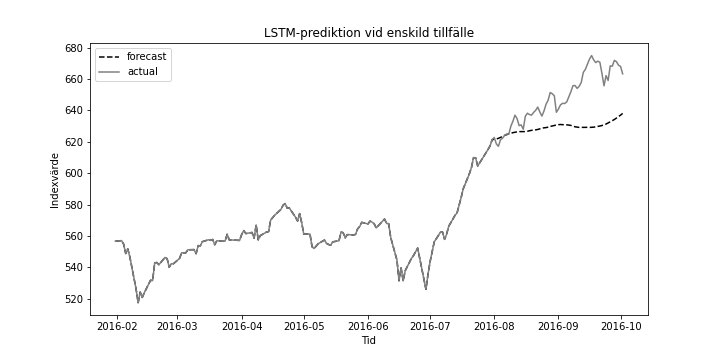
\includegraphics[width=\linewidth]{lstm_pred.png}
\centering
\end{figure}
Notera att LSTM inte har konfidensintervall.

\begin{figure}[H]
\caption{ARMA-GARCH-prediktioner vid enskild tidpunkt}
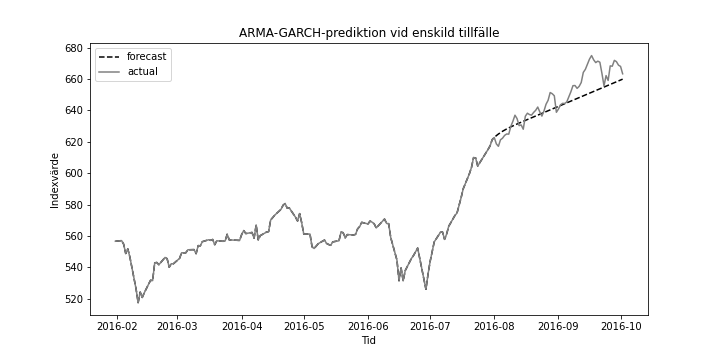
\includegraphics[width=\linewidth]{arma_garch_pred.png}
\centering
\end{figure}

\begin{figure}[H]
\caption{ARMA-GARCH-prediktioner 5 perioder fram vid enskild tidpunkt med prediktionsintervall}
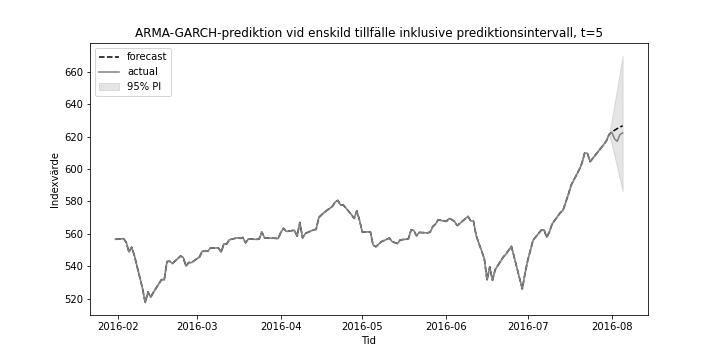
\includegraphics[width=\linewidth]{arma_garch_pred_interval_5.png}
\centering
\end{figure}

\begin{figure}[H]
\caption{ARMA-GARCH-prediktioner 63 perioder fram vid enskild tidpunkt med prediktionsintervall}
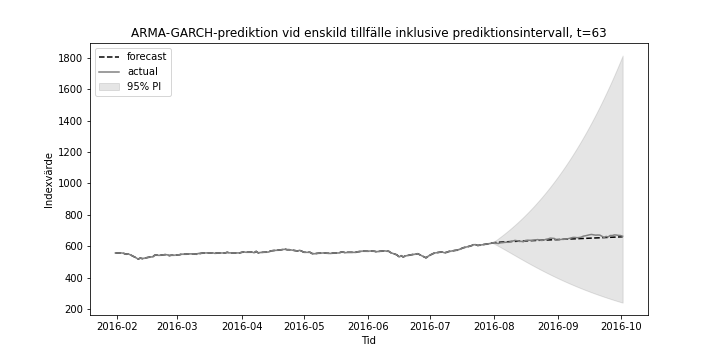
\includegraphics[width=\linewidth]{arma_garch_pred_interval_63.png}
\centering
\end{figure}
Notera hur prediktionsintervallen ska 63 perioder framåt är enorma jämfört med 5 perioder framåt. Detta beror såklart på enormt stora osäkerheter vid så långa prediktioner.

\subsection{AIC och BIC för ett urval av modeller}
Ju lägre värde, desto bättre. ARMA(1,1)-GARCH(1,1) ger lägst resultat.

\begin{table}[H]
\caption{Specifikationer för ARMA-GARCH: AIC \& BIC}
\begin{tabularx}{\textwidth}{c *{6}{Y}}
\toprule
Modell  & AIC & BIC  \\
\hline

ARMA(0,0)-GARCH(1,0)            & -6,782                &   -6,777     \\

ARMA(0,0)-GARCH(1,1)            & -6,938         & -6,931    \\


ARMA(0,1)-GARCH(1,1)            & -6,951         & -6,942   \\

ARMA(1,0)-GARCH(1,1)           & -6,954         & -6,944   \\


\textbf{ARMA(1,1)-GARCH(1,1)}           & \textbf{-6,965}          & \textbf{-6,954}
    \\ 

ARMA(1,1)-GARCH(2,1)           & -6,965         & -6,952   \\ 

ARMA(1,1)-GARCH(2,2)           & -6,964        & -6,950
   \\ 

ARMA(2,1)-GARCH(2,2)           &-6,964        & -6,948    \\ 

ARMA(2,2)-GARCH(2,2)           & -6,963         &  -6,946
   \\ 

\bottomrule
\end{tabularx}
\end{table}

\subsection{Histogram över logaritmerad avkastning}
\begin{figure}[H]
\caption{Histogram logaritmerad avkastning}
\includegraphics[width=\linewidth]{histogram.png}
\centering
\end{figure}



\end{document}